

\documentclass[english]{article}\usepackage[]{graphicx}\usepackage[]{color}
%% maxwidth is the original width if it is less than linewidth
%% otherwise use linewidth (to make sure the graphics do not exceed the margin)
\makeatletter
\def\maxwidth{ %
  \ifdim\Gin@nat@width>\linewidth
    \linewidth
  \else
    \Gin@nat@width
  \fi
}
\makeatother

\definecolor{fgcolor}{rgb}{0.345, 0.345, 0.345}
\newcommand{\hlnum}[1]{\textcolor[rgb]{0.686,0.059,0.569}{#1}}%
\newcommand{\hlstr}[1]{\textcolor[rgb]{0.192,0.494,0.8}{#1}}%
\newcommand{\hlcom}[1]{\textcolor[rgb]{0.678,0.584,0.686}{\textit{#1}}}%
\newcommand{\hlopt}[1]{\textcolor[rgb]{0,0,0}{#1}}%
\newcommand{\hlstd}[1]{\textcolor[rgb]{0.345,0.345,0.345}{#1}}%
\newcommand{\hlkwa}[1]{\textcolor[rgb]{0.161,0.373,0.58}{\textbf{#1}}}%
\newcommand{\hlkwb}[1]{\textcolor[rgb]{0.69,0.353,0.396}{#1}}%
\newcommand{\hlkwc}[1]{\textcolor[rgb]{0.333,0.667,0.333}{#1}}%
\newcommand{\hlkwd}[1]{\textcolor[rgb]{0.737,0.353,0.396}{\textbf{#1}}}%
\let\hlipl\hlkwb

\usepackage{framed}
\makeatletter
\newenvironment{kframe}{%
 \def\at@end@of@kframe{}%
 \ifinner\ifhmode%
  \def\at@end@of@kframe{\end{minipage}}%
  \begin{minipage}{\columnwidth}%
 \fi\fi%
 \def\FrameCommand##1{\hskip\@totalleftmargin \hskip-\fboxsep
 \colorbox{shadecolor}{##1}\hskip-\fboxsep
     % There is no \\@totalrightmargin, so:
     \hskip-\linewidth \hskip-\@totalleftmargin \hskip\columnwidth}%
 \MakeFramed {\advance\hsize-\width
   \@totalleftmargin\z@ \linewidth\hsize
   \@setminipage}}%
 {\par\unskip\endMakeFramed%
 \at@end@of@kframe}
\makeatother

\definecolor{shadecolor}{rgb}{.97, .97, .97}
\definecolor{messagecolor}{rgb}{0, 0, 0}
\definecolor{warningcolor}{rgb}{1, 0, 1}
\definecolor{errorcolor}{rgb}{1, 0, 0}
\newenvironment{knitrout}{}{} % an empty environment to be redefined in TeX

\usepackage{alltt} % \documentclass[a4paper]{article}
\usepackage[T1]{fontenc}
\usepackage[latin9]{inputenc} % \usepackage[utf8]{inputenc}
\usepackage{geometry}
% \geometry{verbose,tmargin=2cm,bmargin=2cm,lmargin=3cm,rmargin=3cm}
\usepackage{amsthm, amsmath,amssymb} % ,amsfonts
\usepackage{setspace}
\usepackage{esint}
\usepackage[authoryear]{natbib}
\onehalfspacing

\makeatletter
\usepackage{authblk}
\usepackage[multiple]{footmisc}
\usepackage{pdflscape}
\usepackage{booktabs}

% \usepackage{jheppub}
%%\usepackage[round]{natbib}
\usepackage[colorlinks=true,urlcolor=blue]{hyperref}
\usepackage{graphicx}
\usepackage{pdflscape}
\usepackage{color}
\usepackage{float}

\definecolor{blue}{rgb}{.2,.2,.7}
\definecolor{red}{rgb}{.7,.2,.2}
\definecolor{green}{rgb}{0,.6,.3}
\definecolor{gray}{rgb}{0.45,0.45,0.45}
\newcommand{\btext}[1]{\textcolor{blue}{#1}}
\newcommand{\rtext}[1]{\textcolor{red}{#1}}
\newcommand{\gtext}[1]{\textcolor{green}{#1}}
\newcommand{\wtext}[1]{\textcolor{white}{#1}}
\newcommand{\old}[1]{\textcolor{gray}{#1}}
\definecolor{gray90}{RGB}{229,229,229}
\definecolor{gray77}{RGB}{196,196,196}
\definecolor{gray60}{RGB}{153,153,153}

\renewcommand{\thefootnote}{\alph{footnote}}
%%\newcommand{\acronym}[1]{\textsc{#1}}
%%\newcommand{\class}[1]{\mbox{\textsf{#1}}}
\newcommand{\code}[1]{\mbox{\texttt{#1}}}
\newcommand{\pkg}[1]{{\normalfont\fontseries{b}\selectfont #1}}
\newcommand{\proglang}[1]{\textsf{#1}}

\newcommand\XOR{\mathbin{\char`\^}}
\newcommand\independent{\protect\mathpalette{\protect\independenT}{\perp}}
\def\independenT#1#2{\mathrel{\rlap{$#1#2$}\mkern2mu{#1#2}}}

\theoremstyle{plain}
\newtheorem*{thm*}{\protect\theoremname}
\theoremstyle{plain}
\newtheorem*{lem*}{\protect\lemmaname}

\makeatother
\usepackage{babel}
\providecommand{\lemmaname}{Lemma}
\providecommand{\theoremname}{Theorem}


%\VignetteEngine{knitr::knitr}
%\VignetteIndexEntry{Introduction}


\IfFileExists{upquote.sty}{\usepackage{upquote}}{}
\begin{document}
\SweaveOpts{concordance=TRUE}



% ------------------------------------------------------------
% \section{Node degree distributions}
% ------------------------------------------------------------



\begin{knitrout}\footnotesize
\definecolor{shadecolor}{rgb}{0.969, 0.969, 0.969}\color{fgcolor}\begin{figure}

{\centering 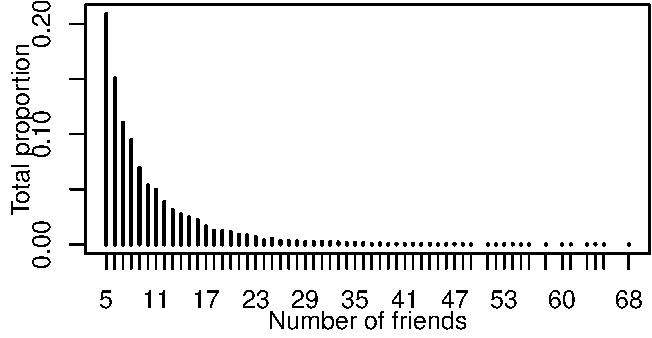
\includegraphics[width=\maxwidth]{TablesFigs/knitR-unnamed-chunk-4-1} 
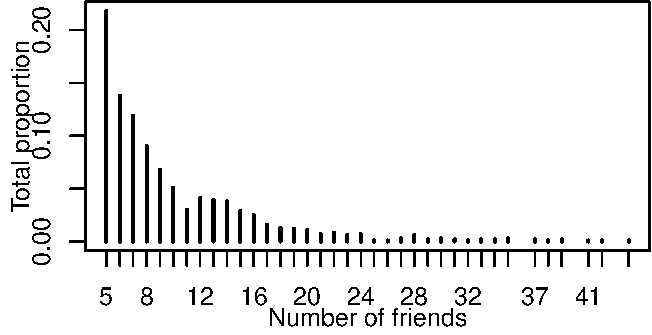
\includegraphics[width=\maxwidth]{TablesFigs/knitR-unnamed-chunk-4-2} 

}

\caption[Node degree distribution for the preferential attachment network with 1,000 (bottom plot) and 10,000 (top plot) observations]{Node degree distribution for the preferential attachment network with 1,000 (bottom plot) and 10,000 (top plot) observations.}\label{fig:unnamed-chunk-4}
\end{figure}


\end{knitrout}




\begin{knitrout}\footnotesize
\definecolor{shadecolor}{rgb}{0.969, 0.969, 0.969}\color{fgcolor}\begin{figure}

{\centering 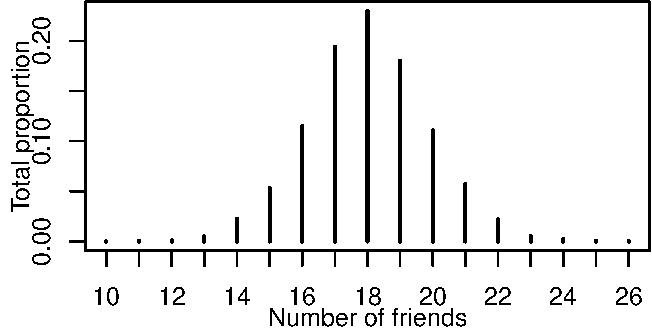
\includegraphics[width=\maxwidth]{TablesFigs/knitR-unnamed-chunk-6-1} 
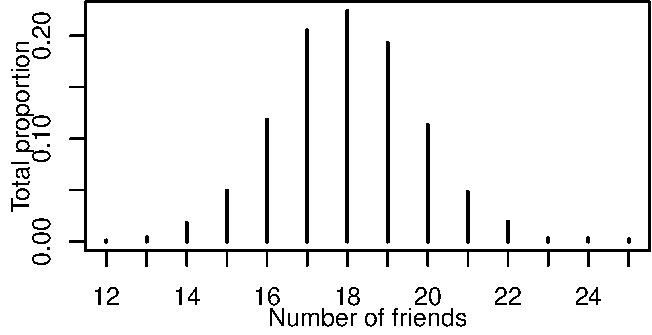
\includegraphics[width=\maxwidth]{TablesFigs/knitR-unnamed-chunk-6-2} 

}

\caption[Node degree distribution for the small world network with 1,000 (bottom plot) and 10,000 (top plot) observations]{Node degree distribution for the small world network with 1,000 (bottom plot) and 10,000 (top plot) observations.}\label{fig:unnamed-chunk-6}
\end{figure}


\end{knitrout}

% ------------------------------------------------------------
% \newpage{}
% \section{Simulation results}
% ------------------------------------------------------------


















% ------------------------------------------------------------------------------------------------------------
\section{Main results}
% ------------------------------------------------------------------------------------------------------------
\begin{knitrout}\footnotesize
\definecolor{shadecolor}{rgb}{0.969, 0.969, 0.969}\color{fgcolor}\begin{figure}

{\centering 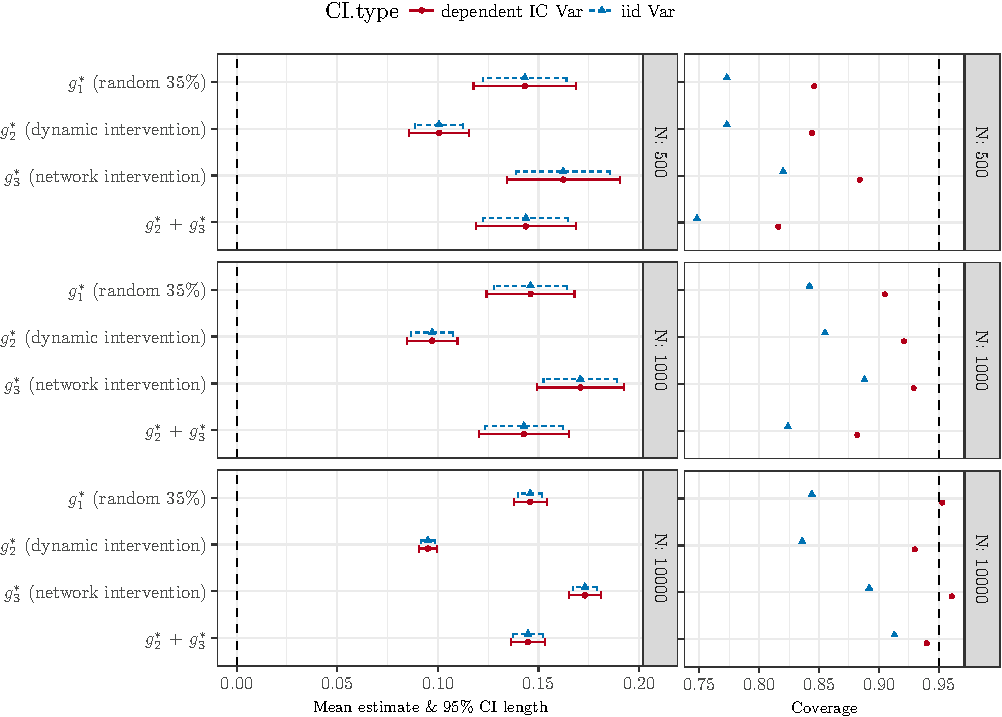
\includegraphics[width=\maxwidth]{TablesFigs/knitR-CIres_EY_prefattach-1} 

}

\caption[Mean 95\% CI length (left panel) and coverage (right panel) for the preferential attachment network, by sample size, interevention and CI type]{Mean 95\% CI length (left panel) and coverage (right panel) for the preferential attachment network, by sample size, interevention and CI type. Results shown for average expected outcomes only.}\label{fig:CIres.EY.prefattach}
\end{figure}


\end{knitrout}

\begin{knitrout}\footnotesize
\definecolor{shadecolor}{rgb}{0.969, 0.969, 0.969}\color{fgcolor}\begin{figure}

{\centering 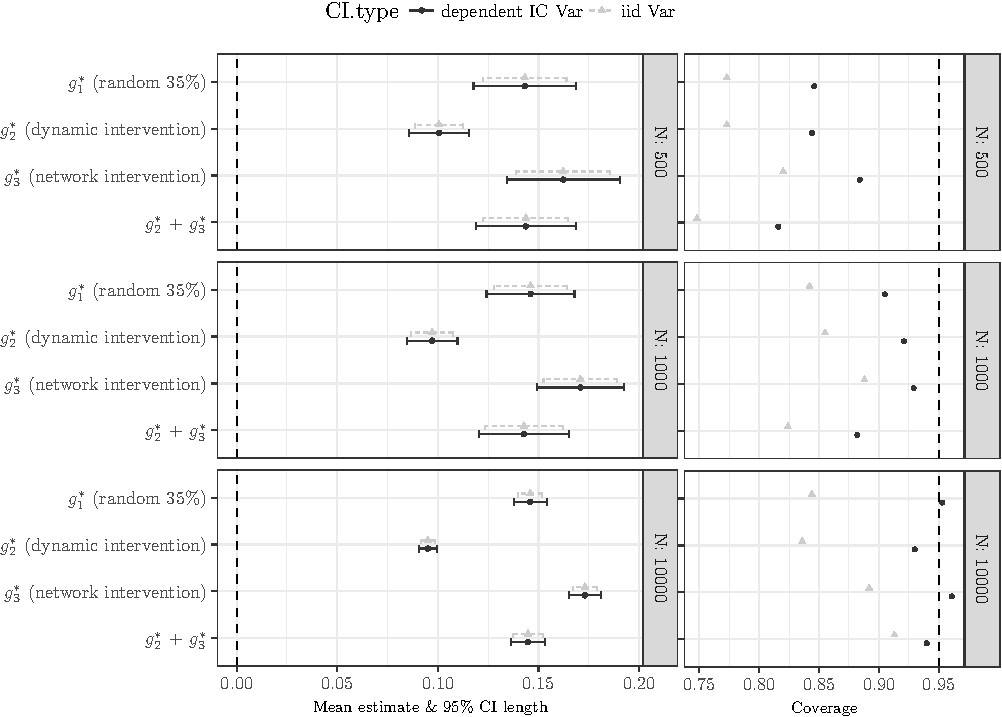
\includegraphics[width=\maxwidth]{TablesFigs/knitR-CIres_EY_prefattach_bw-1} 

}

\caption[Mean 95\% CI length (left panel) and coverage (right panel) for the preferential attachment network, by sample size, interevention and CI type]{Mean 95\% CI length (left panel) and coverage (right panel) for the preferential attachment network, by sample size, interevention and CI type. Results shown for average expected outcomes only.}\label{fig:CIres.EY.prefattach.bw}
\end{figure}


\end{knitrout}

\begin{knitrout}\footnotesize
\definecolor{shadecolor}{rgb}{0.969, 0.969, 0.969}\color{fgcolor}\begin{figure}

{\centering 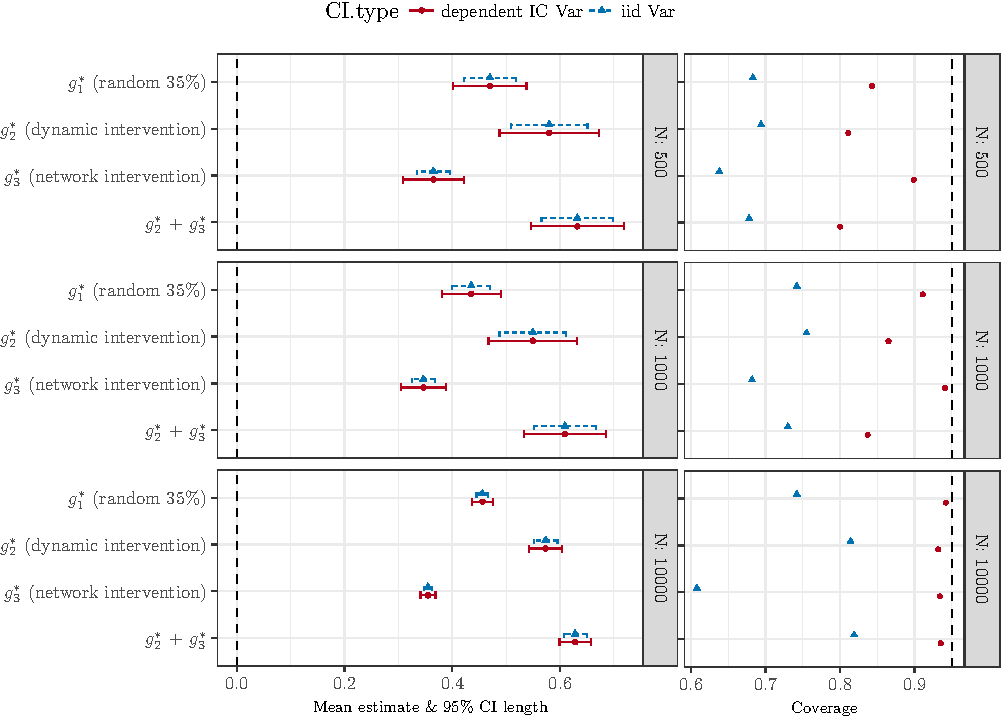
\includegraphics[width=\maxwidth]{TablesFigs/knitR-CIres_EY_smwld-1} 

}

\caption[Mean 95\% CI length (left panel) and coverage (right panel) for the small world network, by sample size, interevention and CI type]{Mean 95\% CI length (left panel) and coverage (right panel) for the small world network, by sample size, interevention and CI type. Results shown for average expected outcomes only.}\label{fig:CIres.EY.smwld}
\end{figure}


\end{knitrout}

\begin{knitrout}\footnotesize
\definecolor{shadecolor}{rgb}{0.969, 0.969, 0.969}\color{fgcolor}\begin{figure}

{\centering 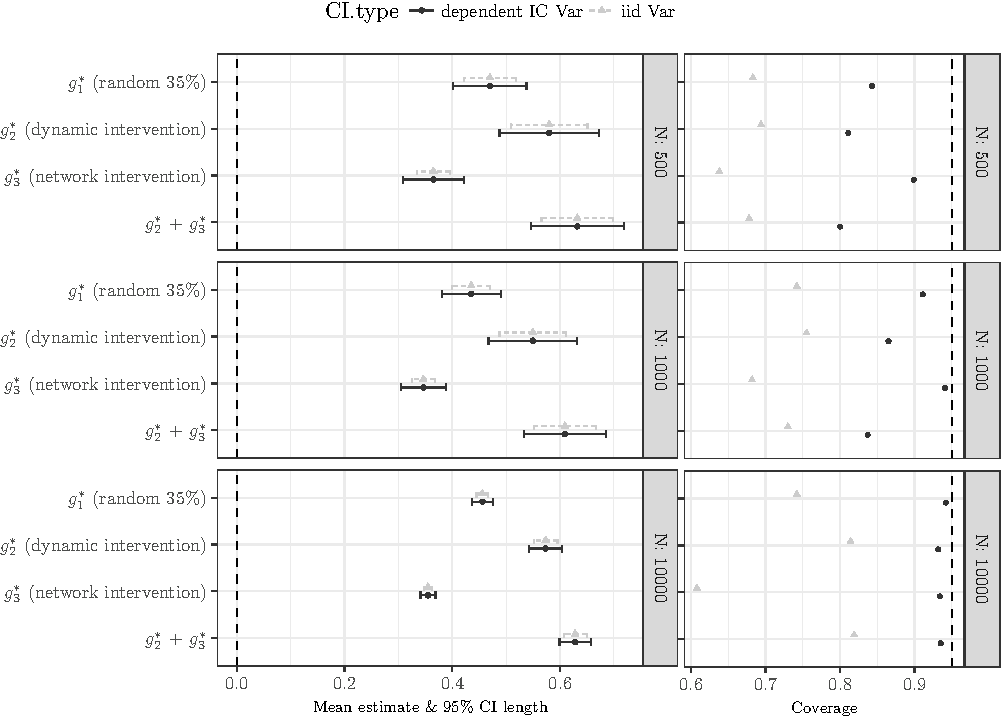
\includegraphics[width=\maxwidth]{TablesFigs/knitR-CIres_EY_smwld_bw-1} 

}

\caption[Mean 95\% CI length (left panel) and coverage (right panel) for the small world network, by sample size, interevention and CI type]{Mean 95\% CI length (left panel) and coverage (right panel) for the small world network, by sample size, interevention and CI type. Results shown for average expected outcomes only.}\label{fig:CIres.EY.smwld.bw}
\end{figure}


\end{knitrout}

\begin{knitrout}\footnotesize
\definecolor{shadecolor}{rgb}{0.969, 0.969, 0.969}\color{fgcolor}\begin{figure}

{\centering 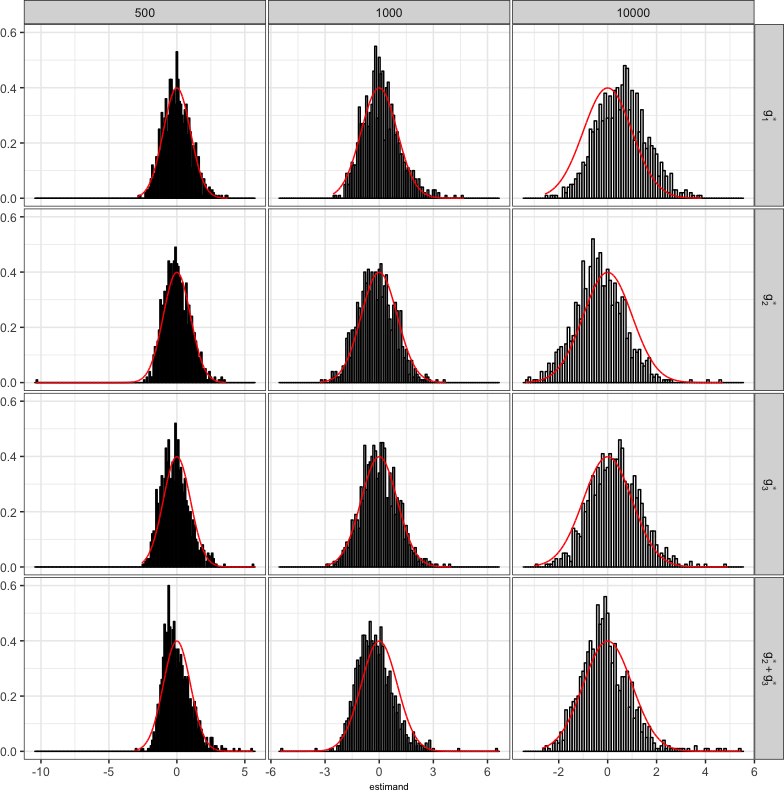
\includegraphics[width=\maxwidth]{TablesFigs/knitR-hist_TMLE_EY_prefattach-1} 

}

\caption[Distribution of the transformed TMLE (black) compared to the theoretical limiting distribution (red) by sample size (x-axis) and intervention type (y-axis)]{Distribution of the transformed TMLE (black) compared to the theoretical limiting distribution (red) by sample size (x-axis) and intervention type (y-axis). The estimates were centered at the truth and re-scaled by true SD. Results shown are for average expected outcomes in the preferential attachment network.}\label{fig:hist.TMLE.EY.prefattach}
\end{figure}


\end{knitrout}

\begin{knitrout}\footnotesize
\definecolor{shadecolor}{rgb}{0.969, 0.969, 0.969}\color{fgcolor}\begin{figure}

{\centering 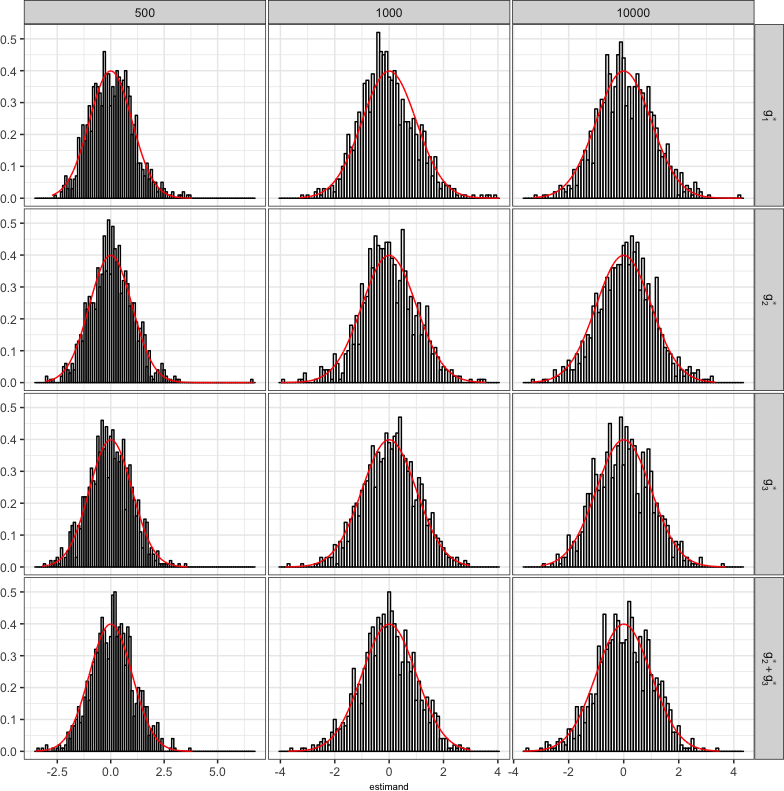
\includegraphics[width=\maxwidth]{TablesFigs/knitR-hist_TMLE_EY_smwld-1} 

}

\caption[Distribution of the transformed TMLE (black) compared to the theoretical limiting distribution (red) by sample size (x-axis) and intervention type (y-axis)]{Distribution of the transformed TMLE (black) compared to the theoretical limiting distribution (red) by sample size (x-axis) and intervention type (y-axis). The estimates were centered at the truth and re-scaled by true SD. Results shown are for average expected outcomes in the small world network.}\label{fig:hist.TMLE.EY.smwld}
\end{figure}


\end{knitrout}

% ------------------------------------------------------------------------------------------------------------
\newpage
\section{Supplementary results}
% ------------------------------------------------------------------------------------------------------------
\begin{knitrout}\footnotesize
\definecolor{shadecolor}{rgb}{0.969, 0.969, 0.969}\color{fgcolor}\begin{figure}

{\centering 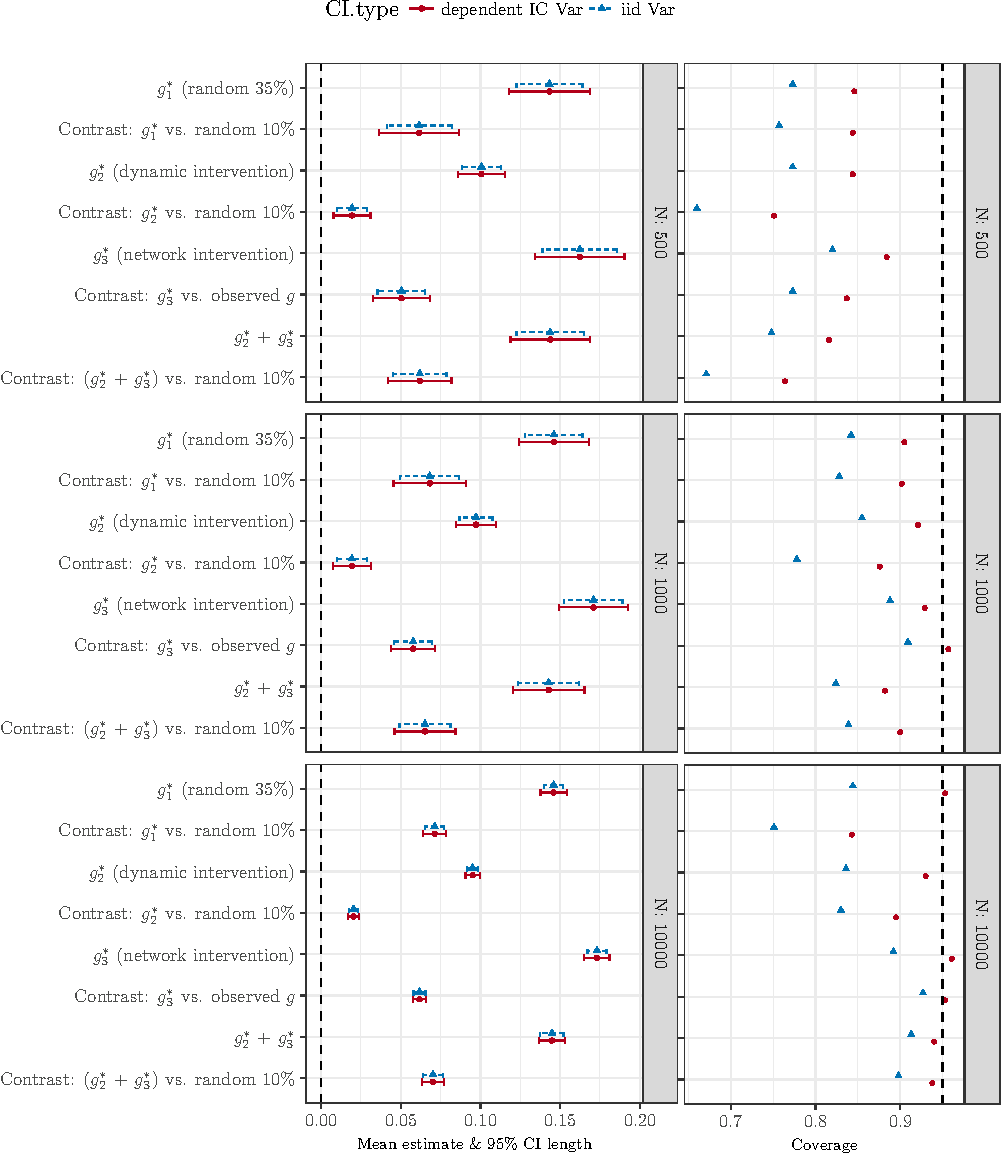
\includegraphics[width=\maxwidth]{TablesFigs/knitR-CIres_ALL_prefattach-1} 

}

\caption[Mean 95\% CI length (left panel) and coverage (right panel) for the preferential attachment network, by sample size, interevention and CI type]{Mean 95\% CI length (left panel) and coverage (right panel) for the preferential attachment network, by sample size, interevention and CI type. Results shown for all scenarios.}\label{fig:CIres.ALL.prefattach}
\end{figure}


\end{knitrout}

\begin{knitrout}\footnotesize
\definecolor{shadecolor}{rgb}{0.969, 0.969, 0.969}\color{fgcolor}\begin{figure}

{\centering 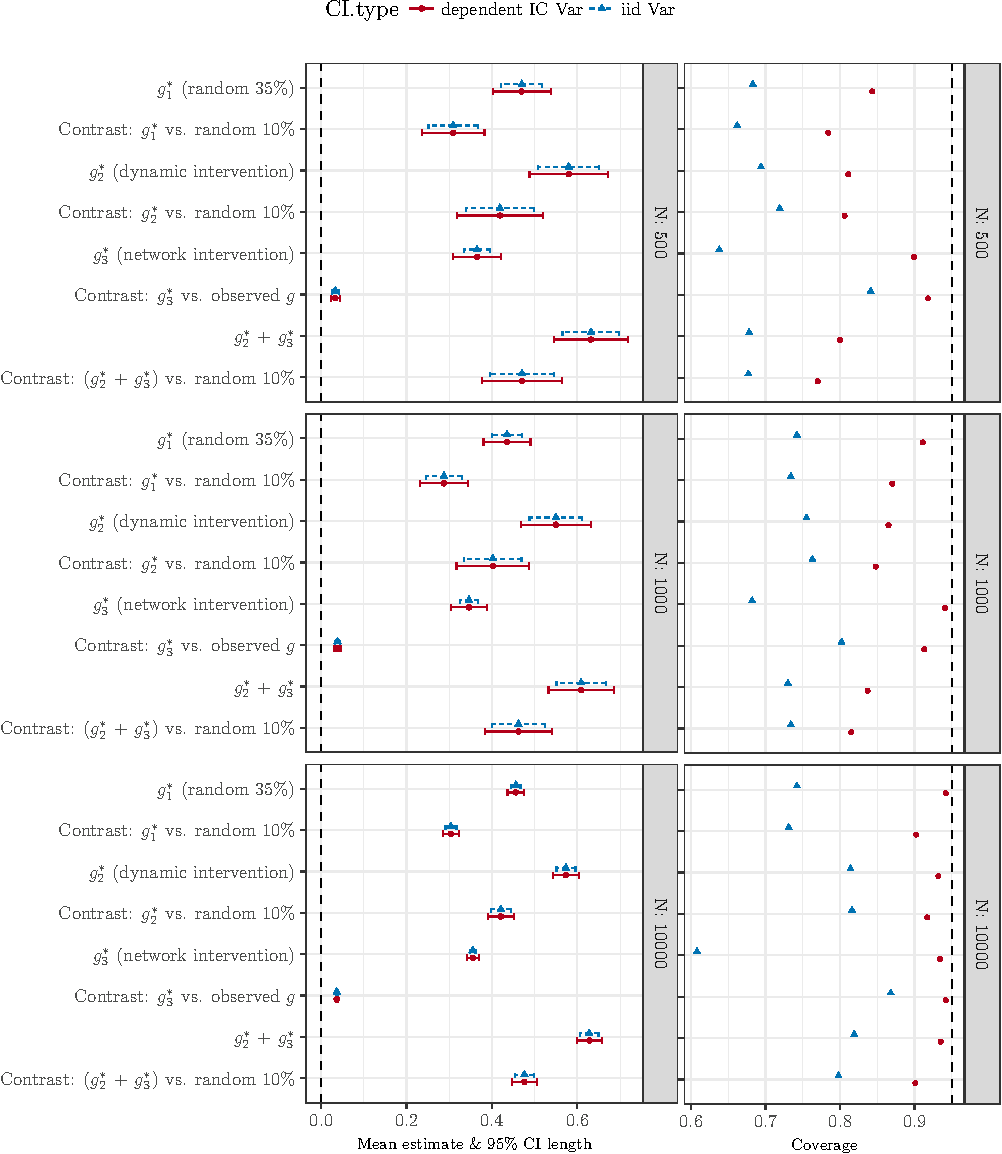
\includegraphics[width=\maxwidth]{TablesFigs/knitR-CIres_ALL_smwld-1} 

}

\caption[Mean 95\% CI length (left panel) and coverage (right panel) for the small world network, by sample size, interevention and CI type]{Mean 95\% CI length (left panel) and coverage (right panel) for the small world network, by sample size, interevention and CI type. Results shown for all scenarios.}\label{fig:CIres.ALL.smwld}
\end{figure}


\end{knitrout}

\begin{knitrout}\footnotesize
\definecolor{shadecolor}{rgb}{0.969, 0.969, 0.969}\color{fgcolor}\begin{figure}

{\centering 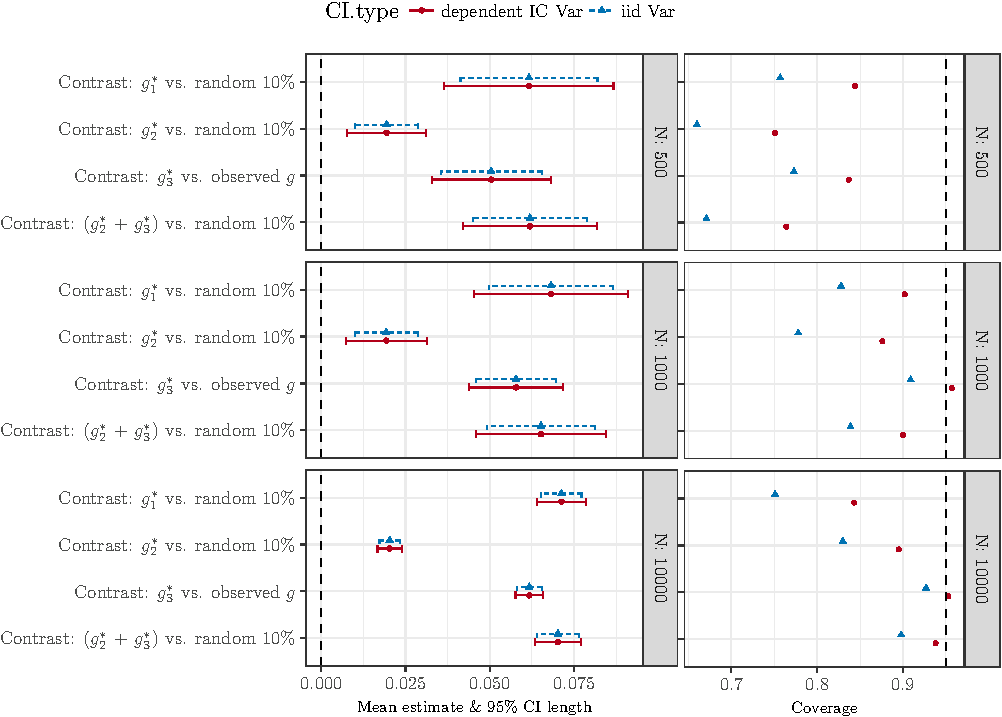
\includegraphics[width=\maxwidth]{TablesFigs/knitR-CIres_ATE_prefattach-1} 

}

\caption[Mean 95\% CI length (left panel) and coverage (right panel) for the preferential attachment network, by sample size, interevention and CI type]{Mean 95\% CI length (left panel) and coverage (right panel) for the preferential attachment network, by sample size, interevention and CI type. Results shown for contrasts only.}\label{fig:CIres.ATE.prefattach}
\end{figure}


\end{knitrout}

\begin{knitrout}\footnotesize
\definecolor{shadecolor}{rgb}{0.969, 0.969, 0.969}\color{fgcolor}\begin{figure}

{\centering 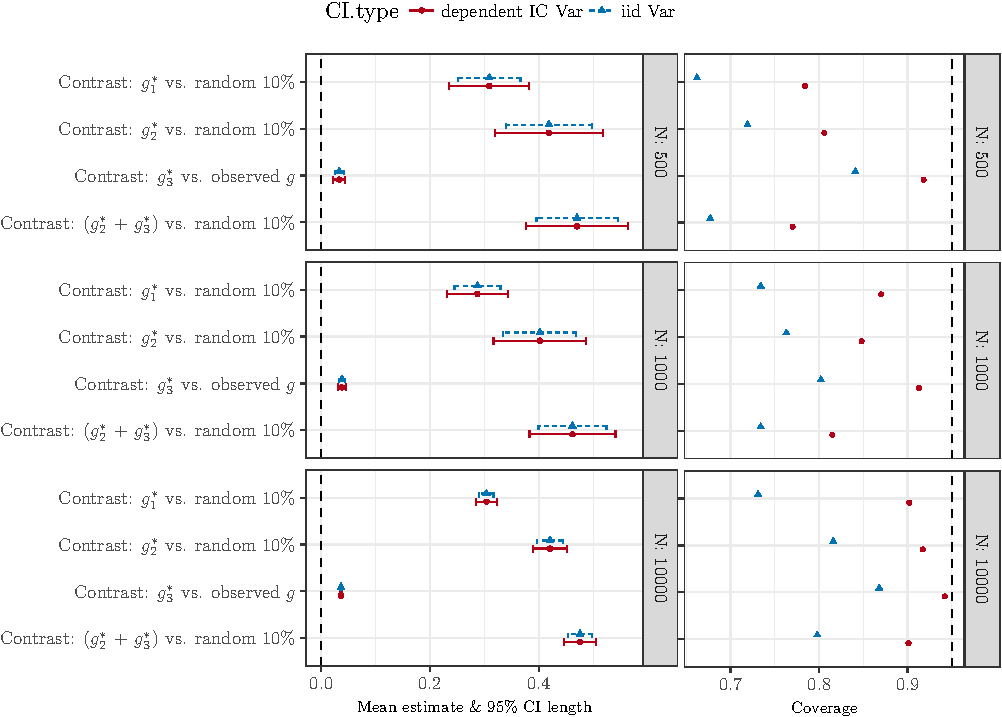
\includegraphics[width=\maxwidth]{TablesFigs/knitR-CIres_ATE_smwld-1} 

}

\caption[Mean 95\% CI length (left panel) and coverage (right panel) for the small world network, by sample size, interevention and CI type]{Mean 95\% CI length (left panel) and coverage (right panel) for the small world network, by sample size, interevention and CI type. Results shown for contrasts only.}\label{fig:CIres.ATE.smwld}
\end{figure}


\end{knitrout}

% ------------------------------------------------------------------------------------------------------------
% TMLE RESULTS (ATE)
% ------------------------------------------------------------------------------------------------------------
\begin{knitrout}\footnotesize
\definecolor{shadecolor}{rgb}{0.969, 0.969, 0.969}\color{fgcolor}\begin{figure}

{\centering 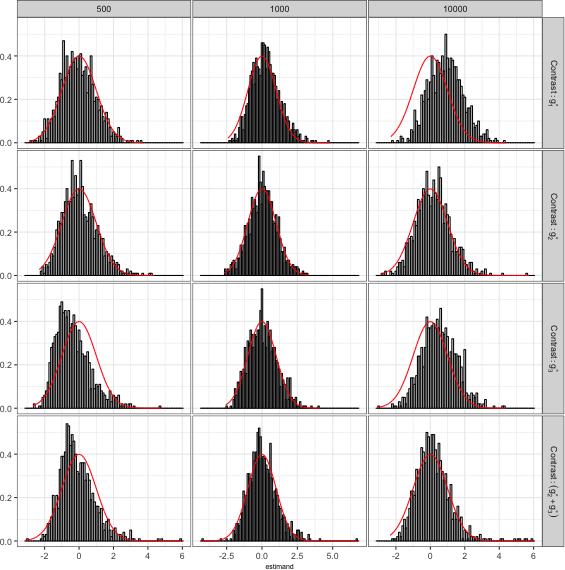
\includegraphics[width=\maxwidth]{TablesFigs/knitR-hist_TMLE_ATE_prefattach-1} 

}

\caption[Distribution of the transformed TMLE (black) compared to the theoretical limiting distribution (red) by sample size (x-axis) and intervention type (y-axis)]{Distribution of the transformed TMLE (black) compared to the theoretical limiting distribution (red) by sample size (x-axis) and intervention type (y-axis). The estimates were centered at the truth and re-scaled by true SD. Results shown are for contrasts in preferential attachment network.}\label{fig:hist.TMLE.ATE.prefattach}
\end{figure}


\end{knitrout}
\begin{knitrout}\footnotesize
\definecolor{shadecolor}{rgb}{0.969, 0.969, 0.969}\color{fgcolor}\begin{figure}

{\centering 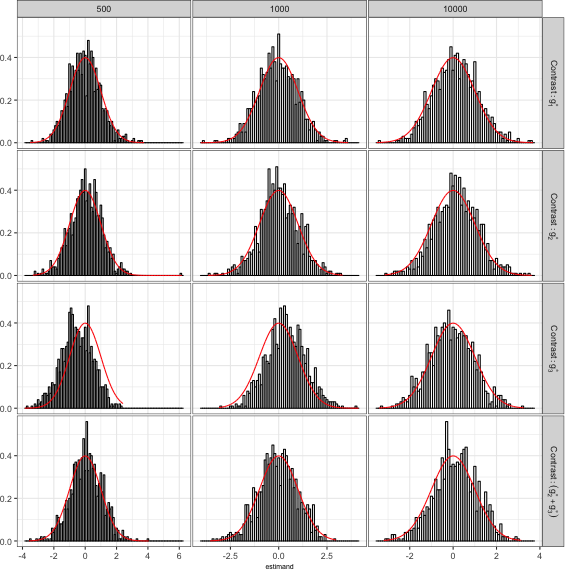
\includegraphics[width=\maxwidth]{TablesFigs/knitR-hist_TMLE_ATE_smwld-1} 

}

\caption[Distribution of the transformed TMLE (black) compared to the theoretical limiting distribution (red) by sample size (x-axis) and intervention type (y-axis)]{Distribution of the transformed TMLE (black) compared to the theoretical limiting distribution (red) by sample size (x-axis) and intervention type (y-axis). The estimates were centered at the truth and re-scaled by true SD. Results shown are for contrasts in small world network.}\label{fig:hist.TMLE.ATE.smwld}
\end{figure}


\end{knitrout}

% ------------------------------------------------------------------------------------------------------------
% IPTW RESULTS (EY and ATE)
% ------------------------------------------------------------------------------------------------------------
\begin{knitrout}\footnotesize
\definecolor{shadecolor}{rgb}{0.969, 0.969, 0.969}\color{fgcolor}\begin{figure}

{\centering 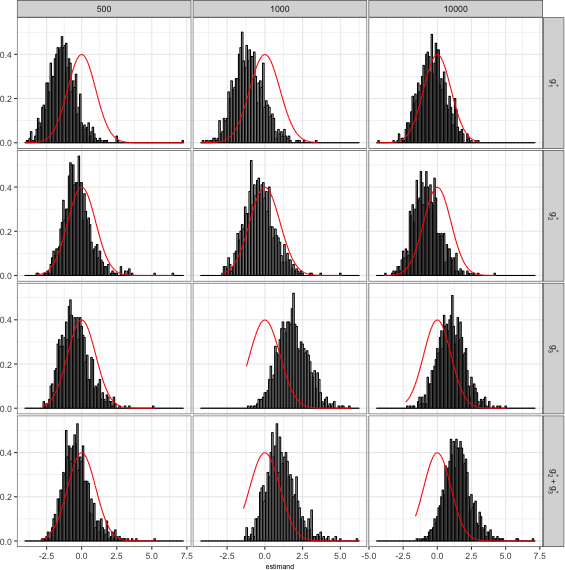
\includegraphics[width=\maxwidth]{TablesFigs/knitR-hist_IPTW_EY_prefattach-1} 

}

\caption[Distribution of the transformed IPTW (black) compared to the theoretical limiting distribution (red) by sample size (x-axis) and intervention type (y-axis)]{Distribution of the transformed IPTW (black) compared to the theoretical limiting distribution (red) by sample size (x-axis) and intervention type (y-axis). The estimates were centered at the truth and re-scaled by true SD. Results shown are for average expected outcomes in the preferential attachment network.}\label{fig:hist.IPTW.EY.prefattach}
\end{figure}


\end{knitrout}

\begin{knitrout}\footnotesize
\definecolor{shadecolor}{rgb}{0.969, 0.969, 0.969}\color{fgcolor}\begin{figure}

{\centering 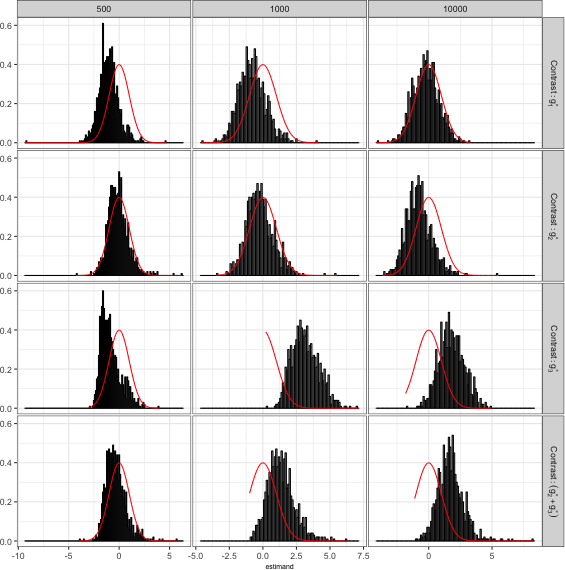
\includegraphics[width=\maxwidth]{TablesFigs/knitR-hist_IPTW_ATE_prefattach-1} 

}

\caption[Distribution of the transformed IPTW (black) compared to the theoretical limiting distribution (red) by sample size (x-axis) and intervention type (y-axis)]{Distribution of the transformed IPTW (black) compared to the theoretical limiting distribution (red) by sample size (x-axis) and intervention type (y-axis). The estimates were centered at the truth and re-scaled by true SD. Results shown are for contrasts in the preferential attachment network.}\label{fig:hist.IPTW.ATE.prefattach}
\end{figure}


\end{knitrout}

\begin{knitrout}\footnotesize
\definecolor{shadecolor}{rgb}{0.969, 0.969, 0.969}\color{fgcolor}\begin{figure}

{\centering 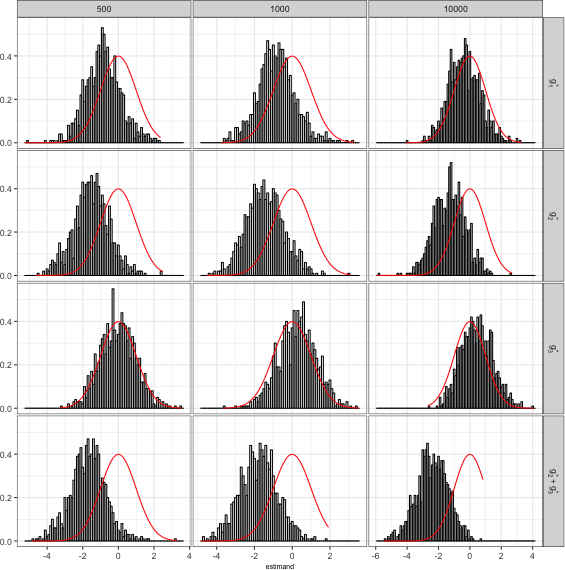
\includegraphics[width=\maxwidth]{TablesFigs/knitR-hist_IPTW_EY_smwld-1} 

}

\caption[Distribution of the transformed IPTW (black) compared to the theoretical limiting distribution (red) by sample size (x-axis) and intervention type (y-axis)]{Distribution of the transformed IPTW (black) compared to the theoretical limiting distribution (red) by sample size (x-axis) and intervention type (y-axis). The estimates were centered at the truth and re-scaled by true SD. Results shown are for average expected outcomes in the small world network.}\label{fig:hist.IPTW.EY.smwld}
\end{figure}


\end{knitrout}

\begin{knitrout}\footnotesize
\definecolor{shadecolor}{rgb}{0.969, 0.969, 0.969}\color{fgcolor}\begin{figure}

{\centering 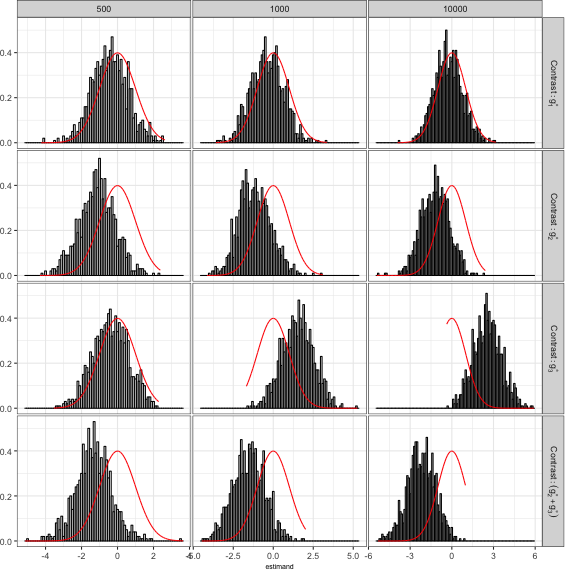
\includegraphics[width=\maxwidth]{TablesFigs/knitR-hist_IPTW_ATE_smwld-1} 

}

\caption[Distribution of the transformed IPTW (black) compared to the theoretical limiting distribution (red) by sample size (x-axis) and intervention type (y-axis)]{Distribution of the transformed IPTW (black) compared to the theoretical limiting distribution (red) by sample size (x-axis) and intervention type (y-axis). The estimates were centered at the truth and re-scaled by true SD. Results shown are for contrasts in the small world network.}\label{fig:hist.IPTW.ATE.smwld}
\end{figure}


\end{knitrout}

\end{document}

